\documentclass{beamer}
\usepackage{booktabs}
\usepackage{xcolor}
\usepackage{changepage}
\usepackage[export]{adjustbox}
\usepackage{booktabs}
\usepackage{graphbox}

\usetheme[numbering=fraction,progressbar=frametitle,sectionpage=none]{metropolis}


% Backup
\newcommand{\backupbegin}{%
   \newcounter{finalframe}
   \setcounter{finalframe}{\value{framenumber}}
}
\newcommand{\backupend}{%
   \setcounter{framenumber}{\value{finalframe}}
}


% Colors
\definecolor{myBlue}{RGB}{21, 56, 110}
\definecolor{myRed}{RGB}{174,0,34}
\definecolor{myRedBg}{RGB}{251, 217, 224}
\definecolor{greySAV}{RGB}{167,166,166}
\definecolor{greyCU}{RGB}{44,46,53}

\setbeamercolor{title}{fg=myBlue}
\setbeamercolor{background canvas}{bg=white}
\setbeamercolor{normal text}{fg=black}
\setbeamercolor{frametitle}{fg=myBlue, bg=white}
\setbeamercolor{section title}{fg=myBlue}
\setbeamercolor{title separator}{fg=myRed,bg=myRedBg}
\setbeamercolor{progress bar}{fg=myRed,bg=myRedBg}
\setbeamercolor{structure}{fg=myRed}


% Thicker progress bar
\makeatletter
\setlength{\metropolis@titleseparator@linewidth}{1pt}
\setlength{\metropolis@progressonsectionpage@linewidth}{1pt}
\setlength{\metropolis@progressinheadfoot@linewidth}{1pt}
\makeatother


% Commands
\newcommand{\bluetext}[1]{%
  \textcolor{myBlue}{#1}
}
\newcommand{\redtext}[1]{%
  \textcolor{myRed}{#1}
}


% Variables
\def\pt{\ensuremath{p_\mathrm{T}}}


% Title
\title[FCCcalo]{FCC-ee: Upstream Correction}
\author[Smiesko, Faltova]{Jana~Faltová\inst{1},
                          Juraj~Smieško\inst{1,2}}
                          % \underline{Juraj~Smieško}\inst{1,2}}
\institute[CU, SAS]{\inst{1} Charles University, Czechia \\
                    \inst{2} Slovak Academy of Sciences, Slovakia}
\date[2020-Dec-03]{\footnotesize
                   Noble Liquid Calorimetry for Future Accelerator
                   Experiments, CERN \\
                   December 17, 2020} % \\
                   % (Ab urbe condita 2773)}


% ---------------------------------------------------------------------------- %
\begin{document}

{%
  \setbeamercolor{background canvas}{bg=greyCU}
  \begin{frame}[noframenumbering]
    \centering
    \vspace{1cm}
    
\includegraphics[width=.25\textwidth]{figures/CU_red_white_logo.pdf}
    \thispagestyle{empty}
  \end{frame}
}

\begin{frame}
  \titlepage{}
  \thispagestyle{empty}
\end{frame}


% \begin{frame}
%   \frametitle{Overview}
%
%   \tableofcontents
% \end{frame}


% ---------------------------------------------------------------------------- %
\section{Upstream Correction}

\begin{frame}
  \frametitle{Upstream Correction}

  Parametrization for FCC-hh:

  \begin{equation*}
  E_\text{upstream} = P_0(E_\text{cluster}, |\eta|) +
                      P_1(E_\text{cluster}, |\eta|) \cdot E_\text{firstLayer}
  \end{equation*}

  \begin{equation*}
    P_0 = P_{00}(|\eta|) + P_{01}(|\eta|) \cdot E_{cluster}  \qquad
    P_1 = P_{10}(|\eta|) + \frac{P_{11}(|\eta|)}{\sqrt{E_{cluster}}}
  \end{equation*}

  % \begin{equation}
  %   E = E_\text{upstream} + E_\text{cluster}
  % \end{equation}

  % \begin{equation}
  %   E_\text{cluster} = \sum_\text{deposits} E_{deposits} \cdot
  %                                           f_\text{sampl}^\text{\,layer}
  % \end{equation}

  % \begin{equation}
  %   E_\text{upstream} = P_{00} + P_{01} \cdot E_\text{cluster} +
  %                       \left( P_{10} + \frac{P_{11}}{\sqrt{E_\text{cluster}}}
  %                       \right) \cdot E_\text{firstLayer}
  % \end{equation}
\end{frame}


\begin{frame}
  \frametitle{P0 and P1 Fit}

  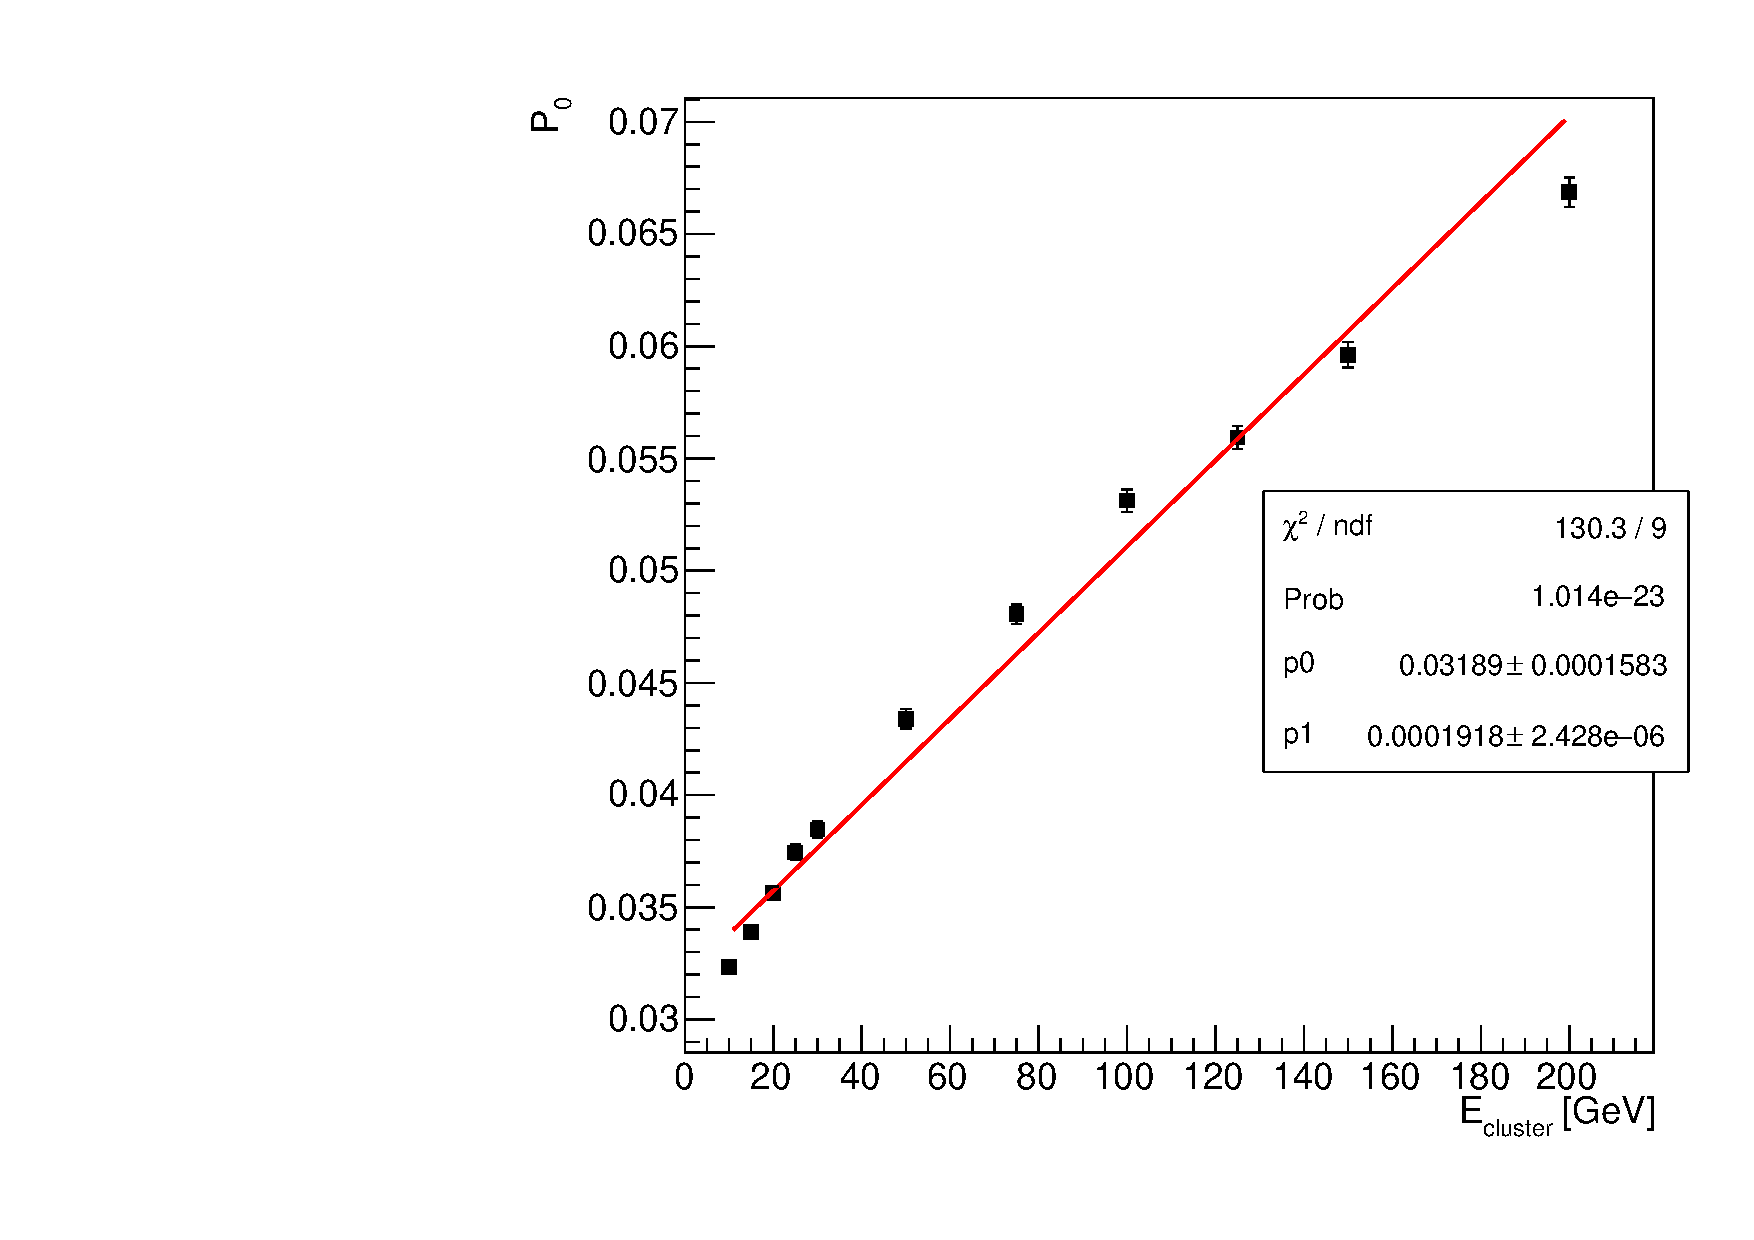
\includegraphics[width=0.49\linewidth]{../../FCC_tools/calo_upstream_corr/output/graph_upstream_corr_param0.pdf}
  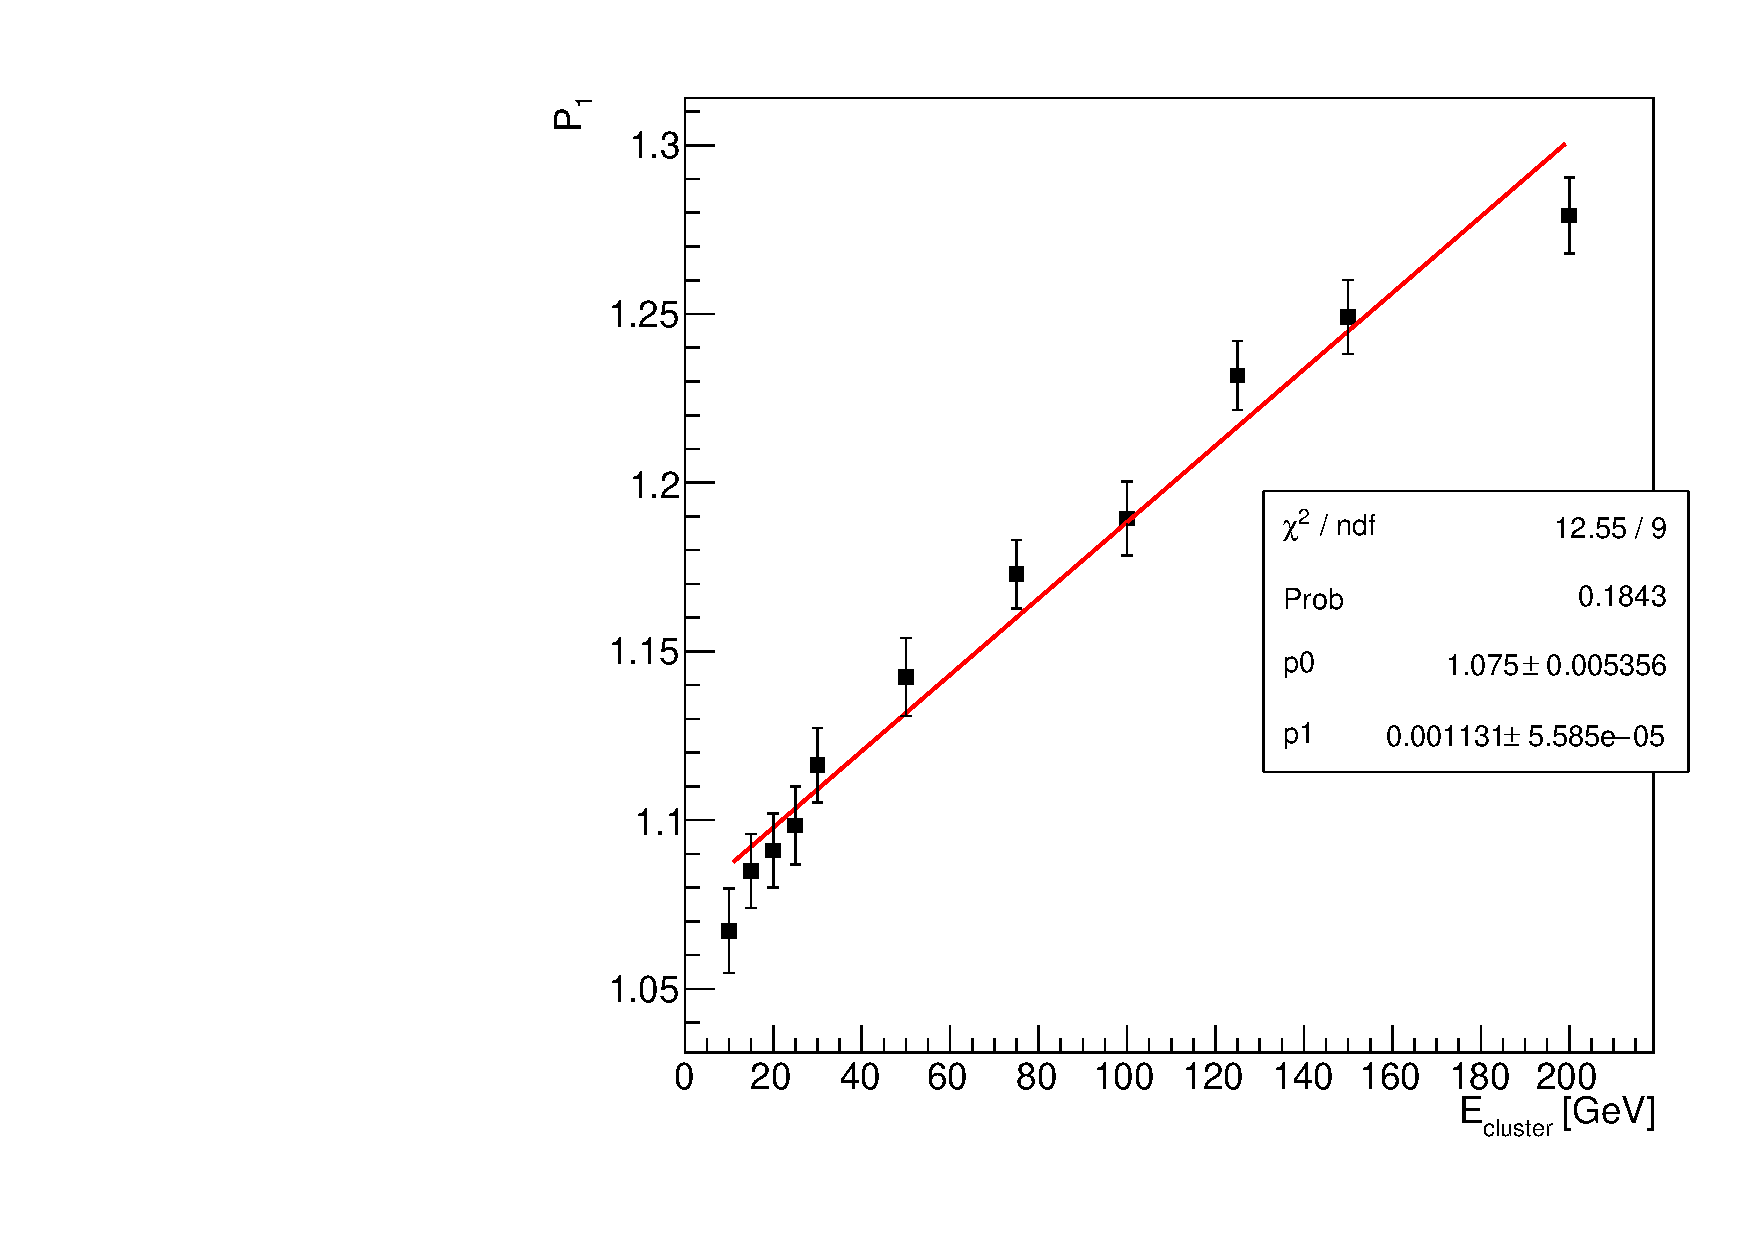
\includegraphics[width=0.49\linewidth]{../../FCC_tools/calo_upstream_corr/output/graph_upstream_corr_param1.pdf}
\end{frame}

\begin{frame}
  \frametitle{At 10 GeV}

  \includegraphics[width=0.49\linewidth]{../../FCC_tools/calo_upstream_corr/output/hist_upstream_vs_first_layer_10GeV.pdf}
  \includegraphics[width=0.49\linewidth]{../../FCC_tools/calo_upstream_corr/output/profile_upstream_vs_first_layer_10GeV.pdf}
\end{frame}


\begin{frame}
  \frametitle{At 15 GeV}

  \includegraphics[width=0.49\linewidth]{../../FCC_tools/calo_upstream_corr/output/hist_upstream_vs_first_layer_15GeV.pdf}
  \includegraphics[width=0.49\linewidth]{../../FCC_tools/calo_upstream_corr/output/profile_upstream_vs_first_layer_15GeV.pdf}
\end{frame}

\begin{frame}
  \frametitle{At 20 GeV}

  \includegraphics[width=0.49\linewidth]{../../FCC_tools/calo_upstream_corr/output/hist_upstream_vs_first_layer_20GeV.pdf}
  \includegraphics[width=0.49\linewidth]{../../FCC_tools/calo_upstream_corr/output/profile_upstream_vs_first_layer_20GeV.pdf}
\end{frame}

\begin{frame}
  \frametitle{At 30 GeV}

  \includegraphics[width=0.49\linewidth]{../../FCC_tools/calo_upstream_corr/output/hist_upstream_vs_first_layer_30GeV.pdf}
  \includegraphics[width=0.49\linewidth]{../../FCC_tools/calo_upstream_corr/output/profile_upstream_vs_first_layer_30GeV.pdf}
\end{frame}

\begin{frame}
  \frametitle{At 50 GeV}

  \includegraphics[width=0.49\linewidth]{../../FCC_tools/calo_upstream_corr/output/hist_upstream_vs_first_layer_50GeV.pdf}
  \includegraphics[width=0.49\linewidth]{../../FCC_tools/calo_upstream_corr/output/profile_upstream_vs_first_layer_50GeV.pdf}
\end{frame}

\begin{frame}
  \frametitle{At 80 GeV}

  \includegraphics[width=0.49\linewidth]{../../FCC_tools/calo_upstream_corr/output/hist_upstream_vs_first_layer_80GeV.pdf}
  \includegraphics[width=0.49\linewidth]{../../FCC_tools/calo_upstream_corr/output/profile_upstream_vs_first_layer_80GeV.pdf}
\end{frame}

\begin{frame}
  \frametitle{At 100 GeV}

  \includegraphics[width=0.49\linewidth]{../../FCC_tools/calo_upstream_corr/output/hist_upstream_vs_first_layer_100GeV.pdf}
  \includegraphics[width=0.49\linewidth]{../../FCC_tools/calo_upstream_corr/output/profile_upstream_vs_first_layer_100GeV.pdf}
\end{frame}

\begin{frame}
  \frametitle{At 120 GeV}

  \includegraphics[width=0.49\linewidth]{../../FCC_tools/calo_upstream_corr/output/hist_upstream_vs_first_layer_120GeV.pdf}
  \includegraphics[width=0.49\linewidth]{../../FCC_tools/calo_upstream_corr/output/profile_upstream_vs_first_layer_120GeV.pdf}
\end{frame}

\begin{frame}
  \frametitle{At 150 GeV}

  \includegraphics[width=0.49\linewidth]{../../FCC_tools/calo_upstream_corr/output/hist_upstream_vs_first_layer_150GeV.pdf}
  \includegraphics[width=0.49\linewidth]{../../FCC_tools/calo_upstream_corr/output/profile_upstream_vs_first_layer_150GeV.pdf}
\end{frame}

\begin{frame}
  \frametitle{At 170 GeV}

  \includegraphics[width=0.49\linewidth]{../../FCC_tools/calo_upstream_corr/output/hist_upstream_vs_first_layer_100GeV.pdf}
  \includegraphics[width=0.49\linewidth]{../../FCC_tools/calo_upstream_corr/output/profile_upstream_vs_first_layer_100GeV.pdf}
\end{frame}

\begin{frame}
  \frametitle{At 100 GeV}

  \includegraphics[width=0.49\linewidth]{../../FCC_tools/calo_upstream_corr/output/hist_upstream_vs_first_layer_170GeV.pdf}
  \includegraphics[width=0.49\linewidth]{../../FCC_tools/calo_upstream_corr/output/profile_upstream_vs_first_layer_170GeV.pdf}
\end{frame}

\begin{frame}
  \frametitle{At 200 GeV}

  \includegraphics[width=0.49\linewidth]{../../FCC_tools/calo_upstream_corr/output/hist_upstream_vs_first_layer_200GeV.pdf}
  \includegraphics[width=0.49\linewidth]{../../FCC_tools/calo_upstream_corr/output/profile_upstream_vs_first_layer_200GeV.pdf}
\end{frame}

\begin{frame}
  \frametitle{At 250 GeV}

  \includegraphics[width=0.49\linewidth]{../../FCC_tools/calo_upstream_corr/output/hist_upstream_vs_first_layer_250GeV.pdf}
  \includegraphics[width=0.49\linewidth]{../../FCC_tools/calo_upstream_corr/output/profile_upstream_vs_first_layer_250GeV.pdf}
\end{frame}

\begin{frame}
  \frametitle{At 300 GeV}

  \includegraphics[width=0.49\linewidth]{../../FCC_tools/calo_upstream_corr/output/hist_upstream_vs_first_layer_300GeV.pdf}
  \includegraphics[width=0.49\linewidth]{../../FCC_tools/calo_upstream_corr/output/profile_upstream_vs_first_layer_300GeV.pdf}
\end{frame}

% ---------------------------------------------------------------------------- %
% \section{Conclusions and Plans}
%
% \begin{frame}
%   \frametitle{Conclusion and Plans}
%
%   \begin{itemize}
%     \item LAr calorimeters were investigated mostly for FCC-hh
%     \item Investigate LAr performance in the FCC-ee framework
%           \begin{itemize}
%             \item Replace existing CLD/IDEA calorimeters with LAr
%           \end{itemize}
%     \item Implement particle flow algorithm for LAr calorimeter
%     \item Multiple R\&D projects directed at LAr at FCC-ee
%   \end{itemize}
% \end{frame}


% \appendix
% \backupbegin{}

% \begin{frame}[c]
%   \begin{center}
%     \redtext{\Huge Backup}
%   \end{center}
% \end{frame}

% \backupend{}

\end{document}
